\documentclass[12pt]{article}
\setlength\parindent{0pt}
\usepackage{fullpage}

\usepackage{amsmath}
\usepackage{graphicx}
\usepackage{color}
\usepackage[margin=2cm]{geometry}
\definecolor{Red}           {rgb}{1,0.3,0.0}
\setlength{\parskip}{4mm}
\def\LL{\left\langle}   % left angle bracket
\def\RR{\right\rangle}  % right angle bracket
\def\LP{\left(}         % left parenthesis
\def\RP{\right)}        % right parenthesis
\def\LB{\left\{}        % left curly bracket
\def\RB{\right\}}       % right curly bracket
\def\PAR#1#2{ {{\partial #1}\over{\partial #2}} }
\def\PARTWO#1#2{ {{\partial^2 #1}\over{\partial #2}^2} }
\def\PARTWOMIX#1#2#3{ {{\partial^2 #1}\over{\partial #2 \partial #3}} }
\newcommand{\BE}{\begin{displaymath}}
	\newcommand{\EE}{\end{displaymath}}
\newcommand{\BNE}{\begin{equation}}
	\newcommand{\ENE}{\end{equation}}
\newcommand{\BEA}{\begin{eqnarray}}
	\newcommand{\EEA}{\nonumber\end{eqnarray}}
\newcommand{\EL}{\nonumber\\}
\newcommand{\la}[1]{\label{#1}}
\newcommand{\ie}{{\em i.e.\ }}
\newcommand{\eg}{{\em e.\,g.\ }}

\newcommand{\cf}{cf.\ }
\newcommand{\etc}{etc.\ }
\newcommand{\Tr}{{\rm tr}}
\newcommand{\etal}{{\it et al.}}
\newcommand{\OL}[1]{\overline{#1}\ } % overline
\newcommand{\OLL}[1]{\overline{\overline{#1}}\ } % double overline
\newcommand{\OON}{\frac{1}{N}} % "one over N"
\newcommand{\OOX}[1]{\frac{1}{#1}} % "one over X"

\begin{document}
		\pagenumbering{gobble}
		\Large
		\centerline{\sc{Recitation Questions}}
		\normalsize
		\centerline{\sc{23 February}}
		
		A penguin slides down a frictionless icy hill; the hill is inclined at an angle $\theta$. In this problem, you will
		calculate the penguin's acceleration. However, I want you to do it two different ways, using two different coordinate systems.
		
		First, solve the problem using the conventional coordinate system, where $x$ is horizontal and $y$ is vertical. As usual, take the following steps:
		
		a) Draw a cartoon of the problem, and label your coordinate system.
		
		{\color{Red}
			They can draw the ramp going either way; that's part of the reason we don't draw it for them. The coordinate system needs to be horizontal/vertical.
		}
	
		
		b) Draw a force diagram for the penguin.
		
		{\color{Red}
			They can either decompose the normal force into components on the diagram or do it somewhere else. The point of having separate (a) and (b) here is to make clear that the force diagram (a bunch of arrows pointing away from a dot) is a separate thing from the cartoon.
}

		c) Write down Newton's second law in both directions -- that is, $\sum F_x = ma_x$ and $\sum F_y = ma_y$. If you have any forces that don't lie along the $x$ or $y$ directions, use trigonometry to break them into components.
		
		
		{\color{Red}
At this point they {\it could} write $a_x$ and $a_y$ as $a \cos \theta$ and $a \sin \theta$ (as Sierra did in the Monday 9:30 staff meeting), but it is more direct to use $a_x$ and $a_y$ here. Note that the only force ``at a funny angle'' is $F_N$.
}
		

		d) This will result in two equations with three unknowns: $a_x$, $a_y$, and $F_N$. However, in this problem, $a_x$ and $a_y$ are related. What is their relation, either to each other or to the magnitude of the acceleration $a$? This should reduce you to two equations and two unknowns; write them below.

{\color{Red}
	They can either do something like $a_x = a \cos \theta$, $a_y = a \sin \theta$ -- or they can write everything in terms of $a_x$, e.g. $a_y = a_x \tan \theta$.
}
		
		e) Solve those equations to find the acceleration of the penguin. Use trigonometry to find the magnitude of $\vec a$.
		
		{\color{Red}
			No matter how they do this, they'll encounter a $\sin^2 \theta + \cos^2 \theta = 1$ identity or similar. The algebra is messy for a little bit until this cancels.
			
			We of course should get $a = g \sin \theta$, maybe with a minus sign depending on coordinate system.
		}
		
		

		Now you will solve the problem again using a rotated coordinate system, where $x$ is the direction parallel to the hill and $y$ is the direction perpendicular to it. Again:
		
		a) Draw a cartoon of the problem, and label your coordinate system.

		
		b) Draw a force diagram for the penguin. (Draw this one large, since you will need to construct a right triangle
		with one of the forces as its hypotenuse to break it into components.)


{\color{Red}
This diagram has the same forces here, but now they need to break the gravitational force into components. Emphasize the language ``component parallel to the ramp'' (this is $x$) and ``component perpendicular to the ramp'' (this is $y$). The most common error here is drawing the $x-$component of gravity parallel to the ground (horizontal).

There are a number of ways to realize that the angle between the gravitational force and the vertical is the same as the angle between the ramp and the horizontal. My favorite is to imagine what happens as the ramp is slowly inclined from flat -- both angles increase from zero.

You can also do high school trig stuff with complements and triangles and stuff.
}
		
		
		c) Write down Newton's second law in both directions -- that is, $\sum F_x = ma_x$ and $\sum F_y = ma_y$.
		If you have any forces that don't lie along the $x$ or $y$ directions, use trigonometry to break them into components.
		This will require some thought: you will need to figure out the components of the
		penguin's weight in the $x$ and $y$ directions. Call over your TA or coach to check your work when you are done.

{\color{Red}
	They may have some stray minus signs floating around depending on their coordinate systems and which way their ramps point, but they should have something like:
	
	\begin{align*}
	\rm X:\hspace{1em}& mg \sin \theta \hspace{1.1cm}= ma_x \\
	\rm Y:\hspace{1em}& F_N - mg \cos \theta = ma_y
	\end{align*}
}
		
		d) This will result in two equations with three unknowns: $a_x$, $a_y$, and $F_N$. However, a little thought will
		tell you what one of these is. What is it? This should reduce you to two equations and two unknowns; write them below.
		
		{\color{Red}
			
			This constraint is again just ``penguin doesn't go through ramp''. It must be the same -- since physics doesn't care about our coordinate system. Earlier it had a complicated mathematical form; now it is just that $a_y=0$.
			
	
			
		}
		
		e) Solve those equations to find the acceleration of the penguin.
		
		{\color{Red}
			Of course we should get the same answer as before: $a = g \sin \theta$.
		}
		
		
		f) Discuss the difference in the two approaches. In one, you aligned your coordinate system with gravity, and in the other, you aligned your coordinate system with the direction that you knew the penguin would accelerate in. Which was easier? Which
		should you adopt for future problems? Invite your TA or coach over to join your conversation.
		
		{\color{Red}
			
			As a matter of course: it is easiest to align your coordinate system {\it with the acceleration}.
			
			A sophisticated perspective is that both our constraint ($\vec a$ must be parallel to ramp), our force diagram, and our equations ($\sum \vec F = m \vec a$) do not care about coordinate systems. We could write
			
			$$\vec F_N + m\vec g = m\vec a$$ 
			
			and then decompose things into components if we wanted. So everything {\it must} be coordinate system invariant. We do this not because it affects the physics, but because it makes the algebra easier.
		}

\begin{center}\underline{\hspace{3in}}\end{center}

		\begin{minipage}{0.7\textwidth}
			Two weights of mass $m_1$ and $m_2$ are attached to either end of a string. This string is passed over a light frictionless pulley, as shown in the image.
			Clearly the heavier mass will go down and the lighter one will go up, but at what rate? In this problem, you will calculate their acceleration.
		\end{minipage} \hfill
		\begin{minipage}{0.3\textwidth}
			\begin{center}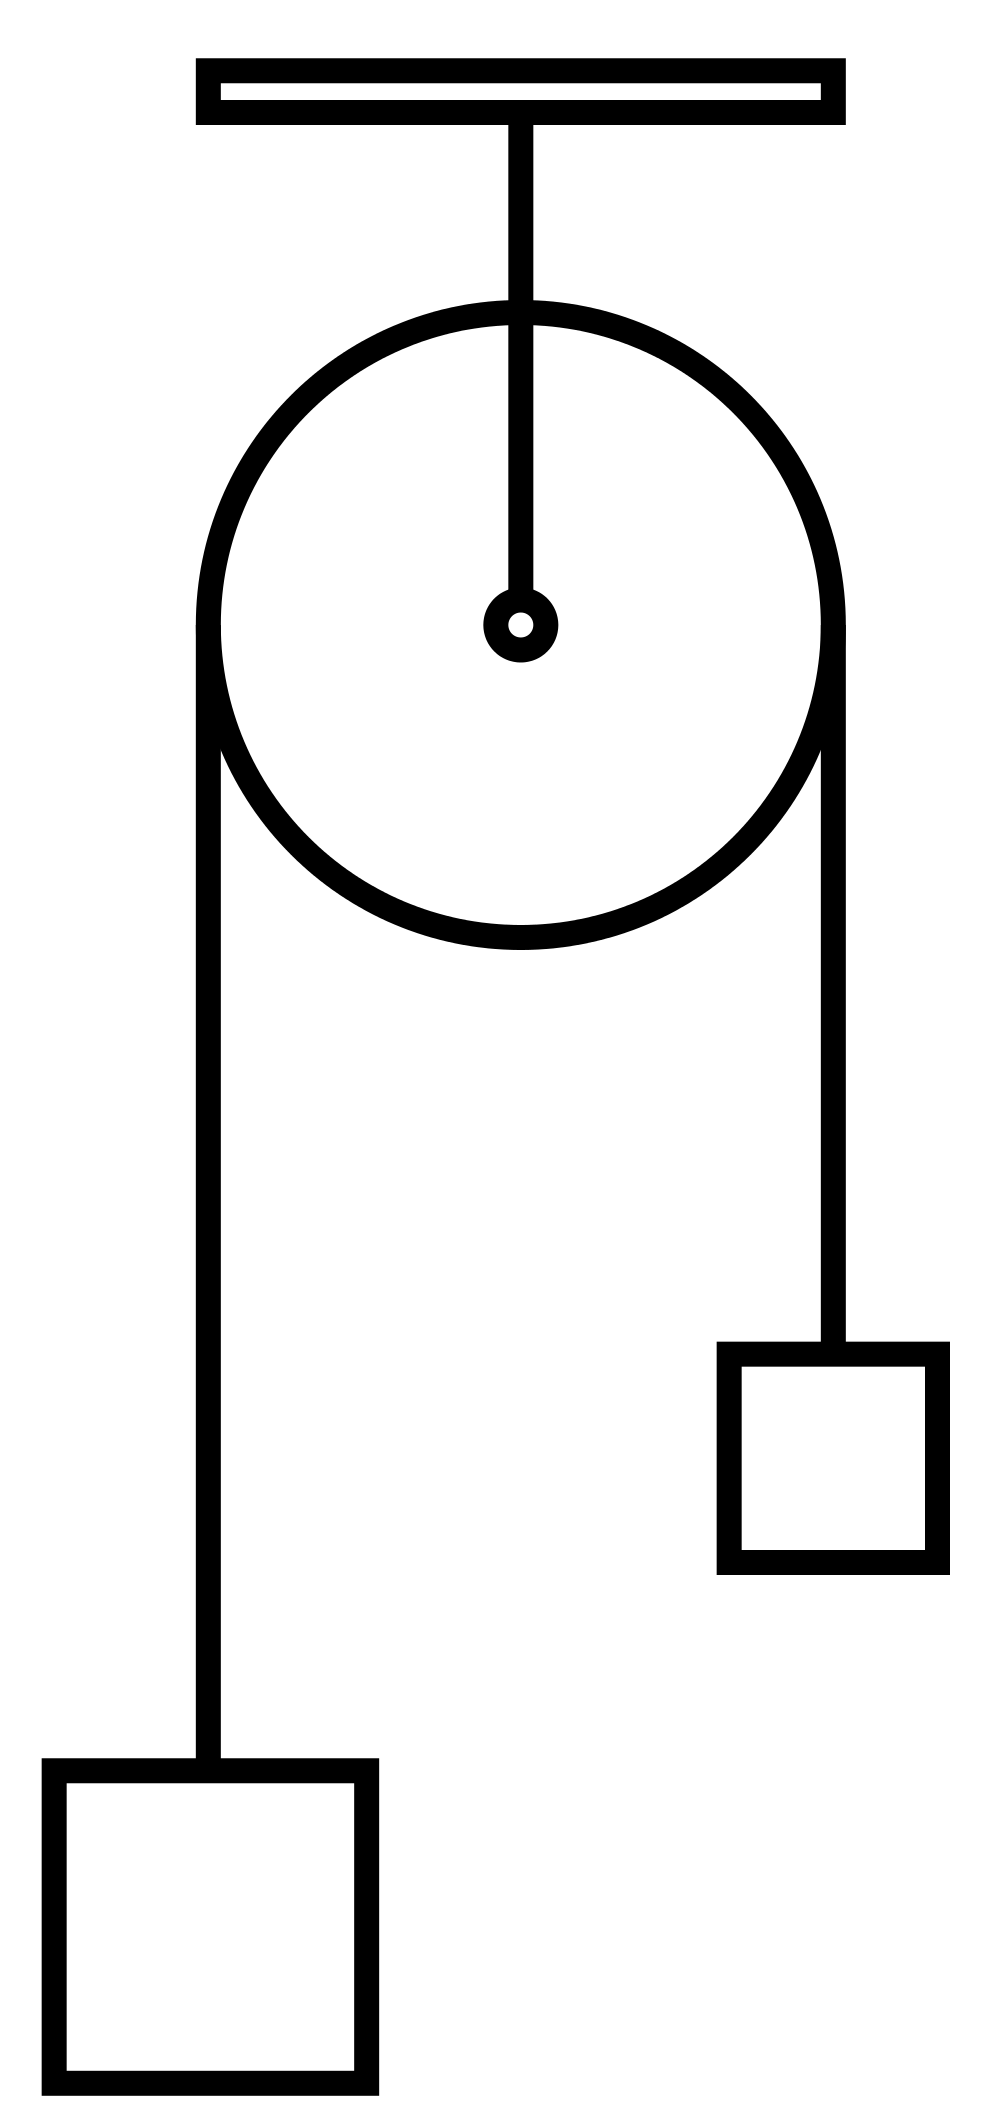
\includegraphics[width=0.5\textwidth]{atwood.png}
			\end{center}
		\end{minipage} \hfill
		
		a) What do you expect the system to do if one of the masses is much heavier than the other? What do you expect if the
		two masses are equal?

{\color{Red}
The good old Atwood machine. If one is much heavier, that one will fall at $g$. Not just ``it will fall'' -- the students should think about its acceleration. As an example, ask them ``What happens if we attach a mouse to an elephant?'' -- obviously the mouse doesn't matter (except to its very small mousy family, so we have to be careful not to squish it and keep it away from the cats in Friday's recitation).
}
		
		
		b) Draw force diagrams for both objects. Label your choice of coordinate system separately for each object -- you don't have to choose the same coordinate system for each!
		
		
		{\color{Red}
			They {\bf should absolutely not} draw a force diagram for ``both objects at once'', with some weird curve to it. This works to find the acceleration -- it doesn't work if we are interested in the tension or anything else.}
		
		
		c) State Newton's law for both objects. Note that their accelerations aren't necessarily the same, depending on your choice of coordinate system, so you should introduce separate variables $a_1$ and $a_2$ for both. The tension forces
		{\it are} the same.
		
				{\color{Red}
					
					This is the most common place to mess this up: anyone blindly using the same $a$ for both objects will mess things up (without flipping the coordinate system for one of them). Some students may want to just remember ``if you have a pulley, choose a coordinate system so you don't have to use two $a$ variables.'' But you can't always do this: there is a double pulley problem on HW4 where the magnitudes aren't equal either.
					
					Encourage them to use separate $a$'s in Newton's second law; they can always set things up ahead of time so they'll work out being equal. But the point is that you have to think about it, not just handwave it and hope you're handwaving in the right direction.
					
					
					
					Some students may ask why the tension is the same. The simplest argument is as follows: we are assuming the string and the pulley are very light. Since $a = \sum F / m$ and $m$ is very small, this means that $\sum F$ must be essentially zero if $a$ isn't going to blow up. And this means that the net force on each little piece of string must be zero, so the tension must be the same everywhere in the string. We don't know about torque yet formally, but you can make a similar argument about the pulley.
				
			
		
	}
				
		
		d) Since you have two objects, you have two copies of Newton's law. However, you have three unknowns: $T$, $a_1$, and $a_2$. What other statement can you make about the accelerations that lets you solve the system?
		
				{\color{Red}
					
					One object goes up and the other object goes down, with the same magnitude. This means $a_1 = \pm a_2$, with the sign depending on coordinate system choice.}
		
		e) Actually solve the system, giving values of $a_1$ and $a_2$ in terms of $m_1$, $m_2$, and $g$. Then, translate
		your expressions for $a_1$ and $a_2$ into words. (Your TA and coaches can help with this.) Does your result make sense?
		Does it agree with your predictions in part (a)?
		
				{\color{Red}
					They should get 
					
					$$ a = \frac{(m_1 - m_2)g}{m_1+m_2}$$
					
					where there may be an overall sign in the numerator. 
		
	\end{document}